The Selection Core is the first of the cores in the genetics accelerator.
It is responsible for selecting appropriate individuals from the rated pool population in the genetics pipeline and pass them on to the other cores so that they may operate on them.

The selection core is designed based on a tournament selection algorithm.
Tournament selection is a selection scheme that aims to quickly find an individual with a high score from an unsorted list in a way that does not guarantee that the selected individual is the one with the highest score.
These goals are healthy goals for a selection algorithm to have when used in a genetic algorithm.

The tournament selection-based selection algorithm is precisely described in algorithm \vref{algorithm:tournament-selection}.
In laymans terms, it is designed to select a single individual from a random position in the rated pool.
The current best and the random selected is compared to each other with use of a comparator.
The best chromosome is stored and used in the next tournament round.
After some number of tournaments the current best is transferred to the crossover core.
The selection core is responsible for letting the rest of the genetic pipeline know when it can fetch the next chromosome. 

\begin{figure}[H]
\begin{algorithm}[H]
\SetAlgoLined
\DontPrintSemicolon
\KwData{$ P = $ A pool of rated individuals, $ r = $ number of rounds in tornament (configurable, $ 0 \le r \le 31 $)}
\KwResult{A selected individual}
\Begin{
    $ k \longleftarrow 0 $\;
    $ bestIndividual \longleftarrow $ random individual from P\;
    \While{$ k < r $}{
        $ individual \longleftarrow $ random individual from P\;
        \If{ $ fitness(individual) > fitness(bestIndividual) $ }{
            $ bestIndividual \longleftarrow individual $\;
        }
        $ k \longleftarrow k + 1 $\;
    }

    \Return{$ bestIndividual $}\;
}
\caption{The tournament selection used in the selection core.}
\label{algorithm:tournament-selection}
\end{algorithm}
\end{figure}

The selection core is designed with efficiency in mind.
The overall time spent in the genetic pipeline must be smaller than the time spent ranking the chromosomes.
Note that the fitness cores are connected to the same memory bus as the genetic pipeline.
This could potentially lead to a memory bottleneck resulting in starvation.
The selection core tries to overcome this fact by reducing the memory access to a minimum.
Note that the selection core has reserved the memory bus during the ongoing tournament.
This implies that port used by the selection core is unavailable to others during this time.
It is designed to not use the memory more than it absolutely have to.
For instance, if the current fitness value is greater than the fitness value just fetched, the selection core will not bother fetching the accompanying chromosome.
This ensures that the memory resources are not wasted, and is accomplished with an \emph{state machine}. 
\todo{show the state machine in a diagram}

Since the Crossover Core will need two inputs when performing crossover, two selection cores are implemented on the genetics pipeline.


\begin{figure}

  \centering
  % Trim er [left bottom right top]
  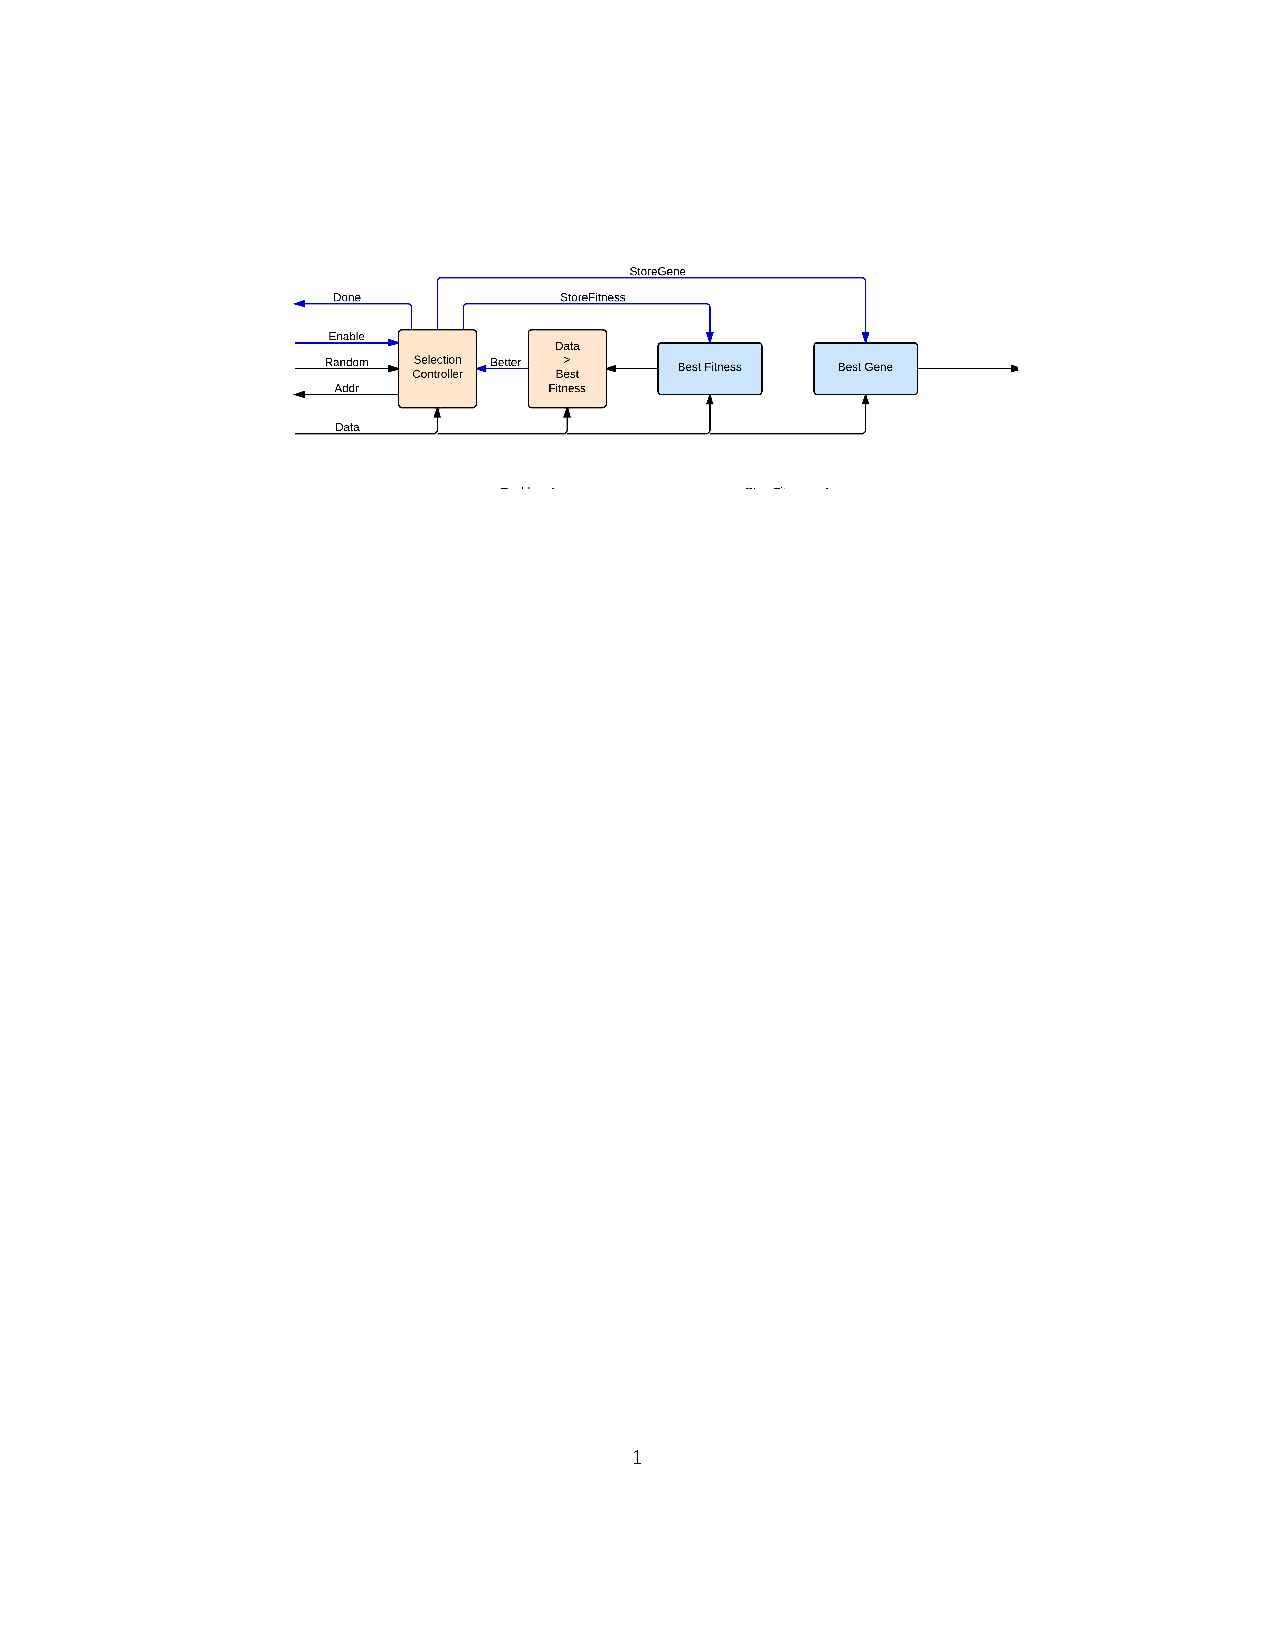
\includegraphics[trim=5cm 20cm 1cm 1cm, clip=true ]{fpga/fig/data_path_selection_core.pdf}
  \caption{Architecture block diagram}
  \label{fpga:fig:selection:selection_core_data_path}
\end{figure}








\begin{figure}

  \centering
  % Trim er [left bottom right top]
  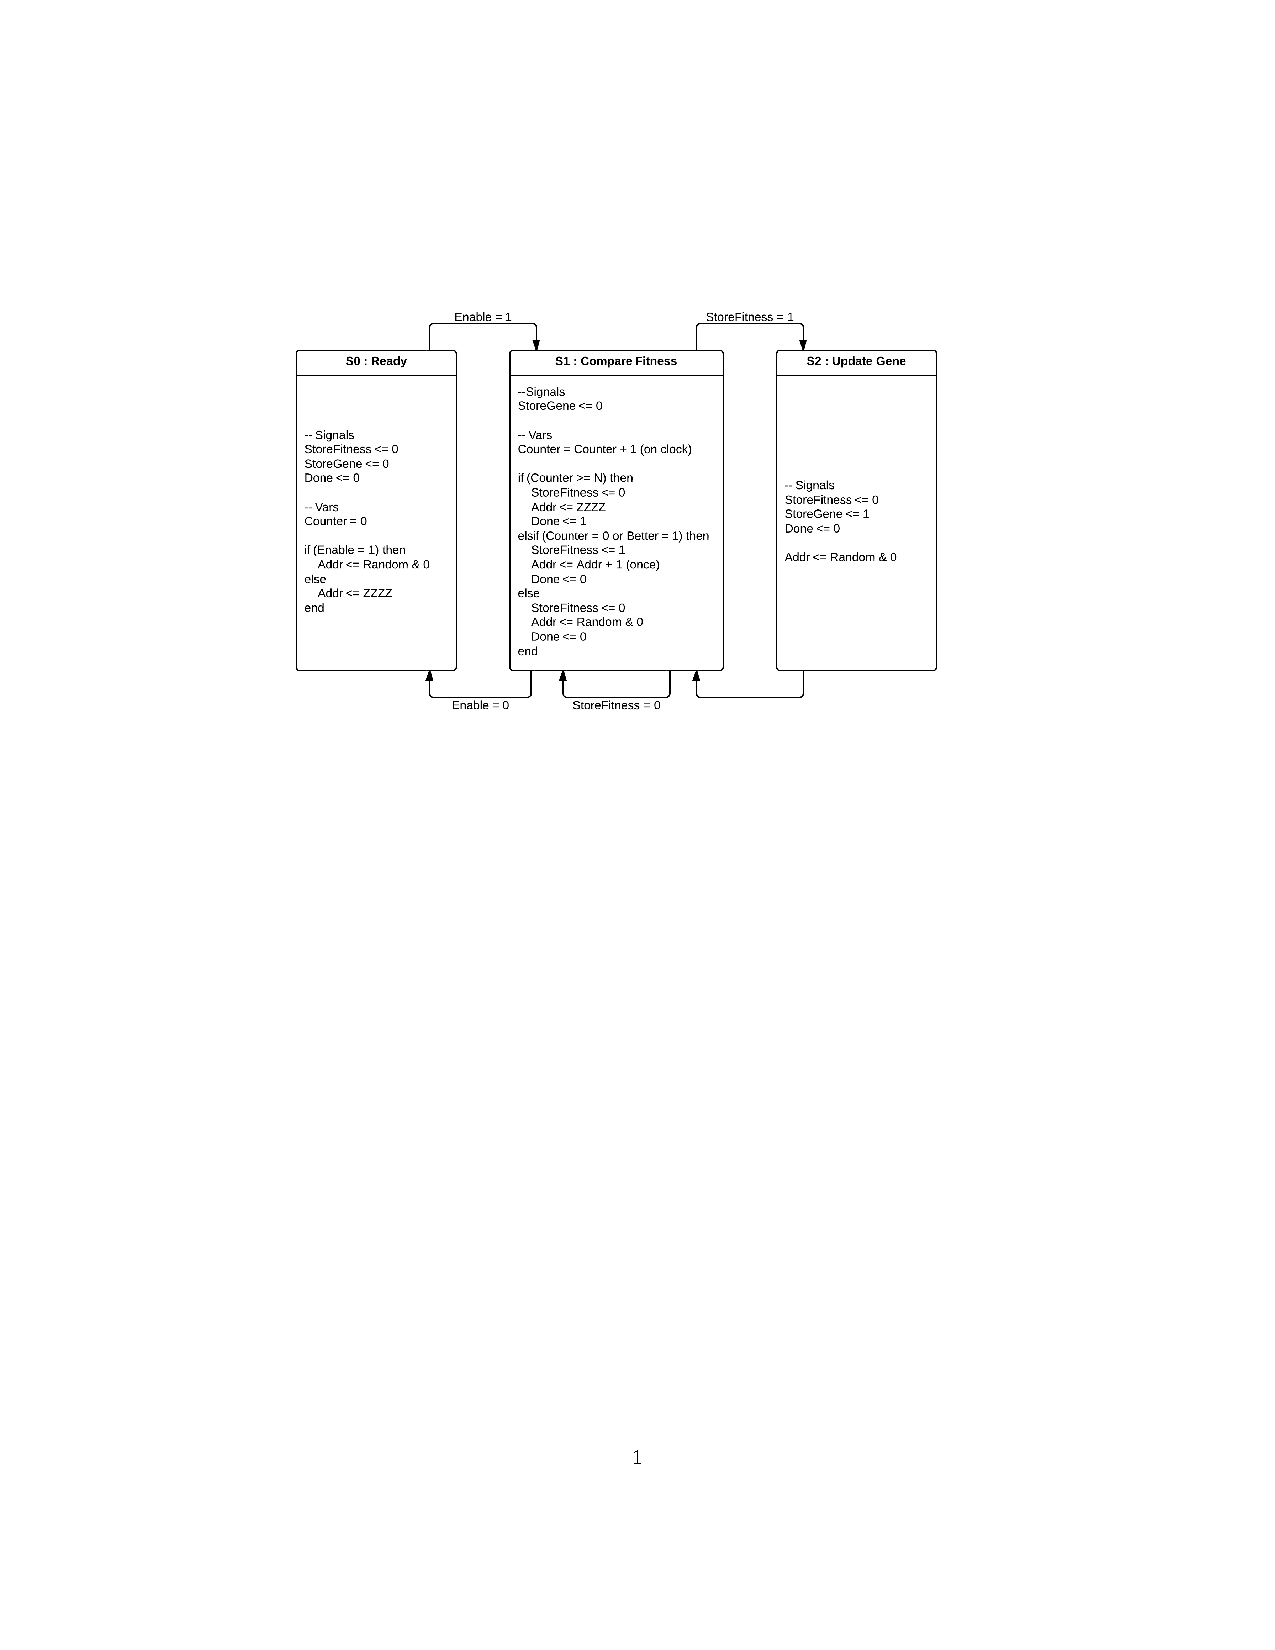
\includegraphics[trim=5cm 16cm 1cm 5cm, clip=true ]{fpga/fig/selection_core_state_machine.pdf}
  \caption{Selection core state machine}
  \label{fpga:fig:selection:selection_core_state_machine}
\end{figure}








